\documentclass{ezb}
\usepackage[]{todonotes}
\usepackage{longtable}
\usepackage{booktabs}

\renewcommand{\thesubsection}{\alph{subsection}}
\begin{document}

% \maketitle{Nummer}{Abgabedatum}{Tutor-Name}{Gruppennummer}
%           {Teilnehmer 1}{Teilnehmer 2}{Teilnehmer 3}
\maketitle{1}{\today}{U. Frese}{}
          {A.O.}{Frank Ihle - 3010158}{Simon Schirrmacher}{N.C.}

%-------Text-Start------------------------------------------
\section{Wer hat mein Tellerchen verrückt? (10 Punkte)}

\newpage
\section{Kekse (4 Punkte)}
Mit der Hilfe der Bildverarbeitung soll eine optische Qualitätskontrolle von einem Butterkeks durchgeführt werden, damit dem Kunden keine Ware mit fehlenden Zähnen oder anderen Verunstaltungen ausgeliefert wird. Abb. \ref{fig:keks_original} zeigt ein Beispiel von einem fehlerfreien Keks, wie es der Konsument erhalten soll.
\begin{figure}[!h]
\begin{center}
    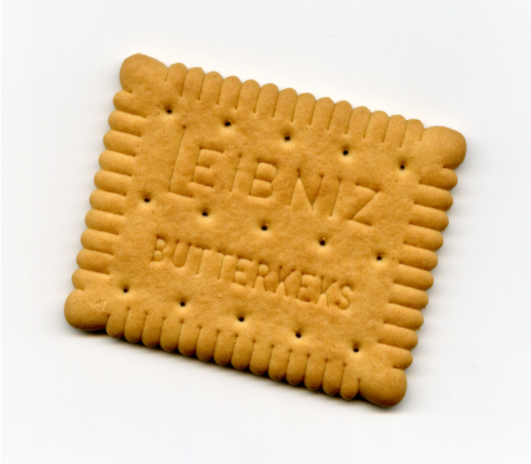
\includegraphics[scale=0.3]{Keks_original.png}
\end{center}
    \caption{Beispiel für einen Keks ohne fehlende Zähne.}
    \label{fig:keks_original}
\end{figure}\\
\newline
\textbf{{\large Fehlererkennung}}\\
\newline
Eine Möglichkeit fehlerbehaftete Ware zu erkennen, kann mit Hilfe eines Vergleichs der Bilder zwischen einem möglichst makellosen Keks (Musterbild) und des zu kontrollierenden Gebäcks (Kontrollbild) erreicht werden.\\
\newline
Zunächst muss die Ware von der Kamera erfasst werden. Hierbei kann es vorkommen, dass der Rand vom Keks nicht parallel zur Bildkante verläuft (vgl. Abb. \ref{fig:keks_original}). Die Aufnahme muss demnach entsprechend gedreht werden, damit beide Kekse miteinander verglichen werden können - ansonsten werden falsche Bereiche miteinander verarbeitet und das Ergebnis ist unbrauchbar. Je nach Fertigungsgenauigkeit kann mit Hilfe der Luftlöchern oder einer Bounding-Box am Keksrand die Orientierung der einzelnen Kekse durchgeführt werden.\\
\newline
Wenn anschließend die Aufnahme bereit zum Vergleich ist, sollen die Pixelwerte beider Bilder voneinander subtrahiert werden. Dadurch lassen sich auf einfache Weise Unterschiede erkennen. Ist beispielsweise das Kontrollbild exakt das Gleiche, wie das Musterbild, so subtrahieren sich für jeden Pixel im Bild immer die selben Werte zu 0 und es entsteht ein schwarzes Bild. Ergeben sich Unterschiede weist das resultierende Bild auf diese Stellen mit anderen Pixelwerten hin. Hierfür bieten sich  verschiedene Varianten an, z.B.:
\begin{equation}
\textbf{R} = \textbf{K} - \textbf{M}
\end{equation}
\textbf{R} $\widehat{=}$ resultierende Bildmatrix, \textbf{K} $\widehat{=}$ Bildmatrix vom Kontrollbild, \textbf{M} $\widehat{=}$ Bildmatrix vom Musterbild. \\
\newline
Wenn nach dieser Variante ein Pixelwert von \textbf{M} größer als der korrespondierende aus \textbf{K} ist, so erhält \textbf{R} einen negativen Wert für diese Stelle. Solche Werte (also $\leq$ 0) können dann auf 0 gesetzt werden. Dies würde aber ein Informationsverlust bedeuten. Stattdessen bleibt die Information erhalten, wenn nach der Subtraktion noch der Betrag gebildet wird:
\begin{equation}
\textbf{R} = \vert \textbf{K} - \textbf{M} \vert 
\end{equation}
Je nach Anforderung kann hier weiter nach Qualitätsstufen unterteilt werden, in z.B.: fehlende Zähne oder Teig, der beim Backen übergelaufen ist. Hierfür müssen dann weitere Klassifizierungsalgorithmen auf \textbf{R} angewendet werden. Üblicherweise soll aber jeder Keks mit irgendeinem Fehler aussortiert werden. Dafür bietet sich ein einfacheres Verfahren an: der Keks soll aussortiert werden, wenn ein bestimmter Helligkeitswert überschritten worden ist, oder wenn dieser Wert eine bestimmte Anzahl überschritten hat (mit Hilfe einer Histogrammanalyse).\\
\textbf{{\large Kamera und Umgebung}}\\
\newline
Für dieses Verfahren ist die beste Kameraposition direkt über dem Mittelpunkt des Gebäcks, da so die meisten Fehler auf der Draufsicht erkannt werden können. Die abzufotografierende Fläche muss beleuchtet werden, um den kompletten Keks analysieren zu können. Die Lichtquelle selbst sollte möglichst nah bei der Kamera platziert werden, um einen Schattenwurf zu vermeiden (ggf. mehrere Lichtquellen verwenden). \\ 
\newline
\textbf{{\large Integration in den Fertigungsprozess}}\\
\newline
Die Kekse werden nacheinander, im Abstand von einer Aufnahmebreite (sodass nur ein Gebäck pro Foto aufgenommen und analysiert wird), mit Hilfe eines Förderbands an der Kamera vorbeigefahren. Um die Bildverarbeitungszeit gering zu halten, kann ein zusätzlicher Sensor (z.B.: Lichtschranke in Richtung der Gebäckkante) die Fotoaufnahme auslösen, wenn der Keks komplett im Bildbereich liegt. Dadurch muss nicht erst überprüft werden, ob das Gebäck komplett oder nur teilweise auf der Aufnahme zu sehen ist. Dieser Sensor kann ebenso zur Synchronisation verwendet werden, indem er die Warenauflage auf das Förderband auslöst. Fehlerbehaftete Kekse können letztlich mit Hilfe von pneumatischen Modulen vom Band geschoben werden.
\newpage
\section{Teller sind ein weites Feld (2 Bonuspunkte)}




%-------Text-End------------------------------------------
\end{document}

